% Created by tikzDevice version 0.7.0 on 2015-01-08 15:16:40
% !TEX encoding = UTF-8 Unicode
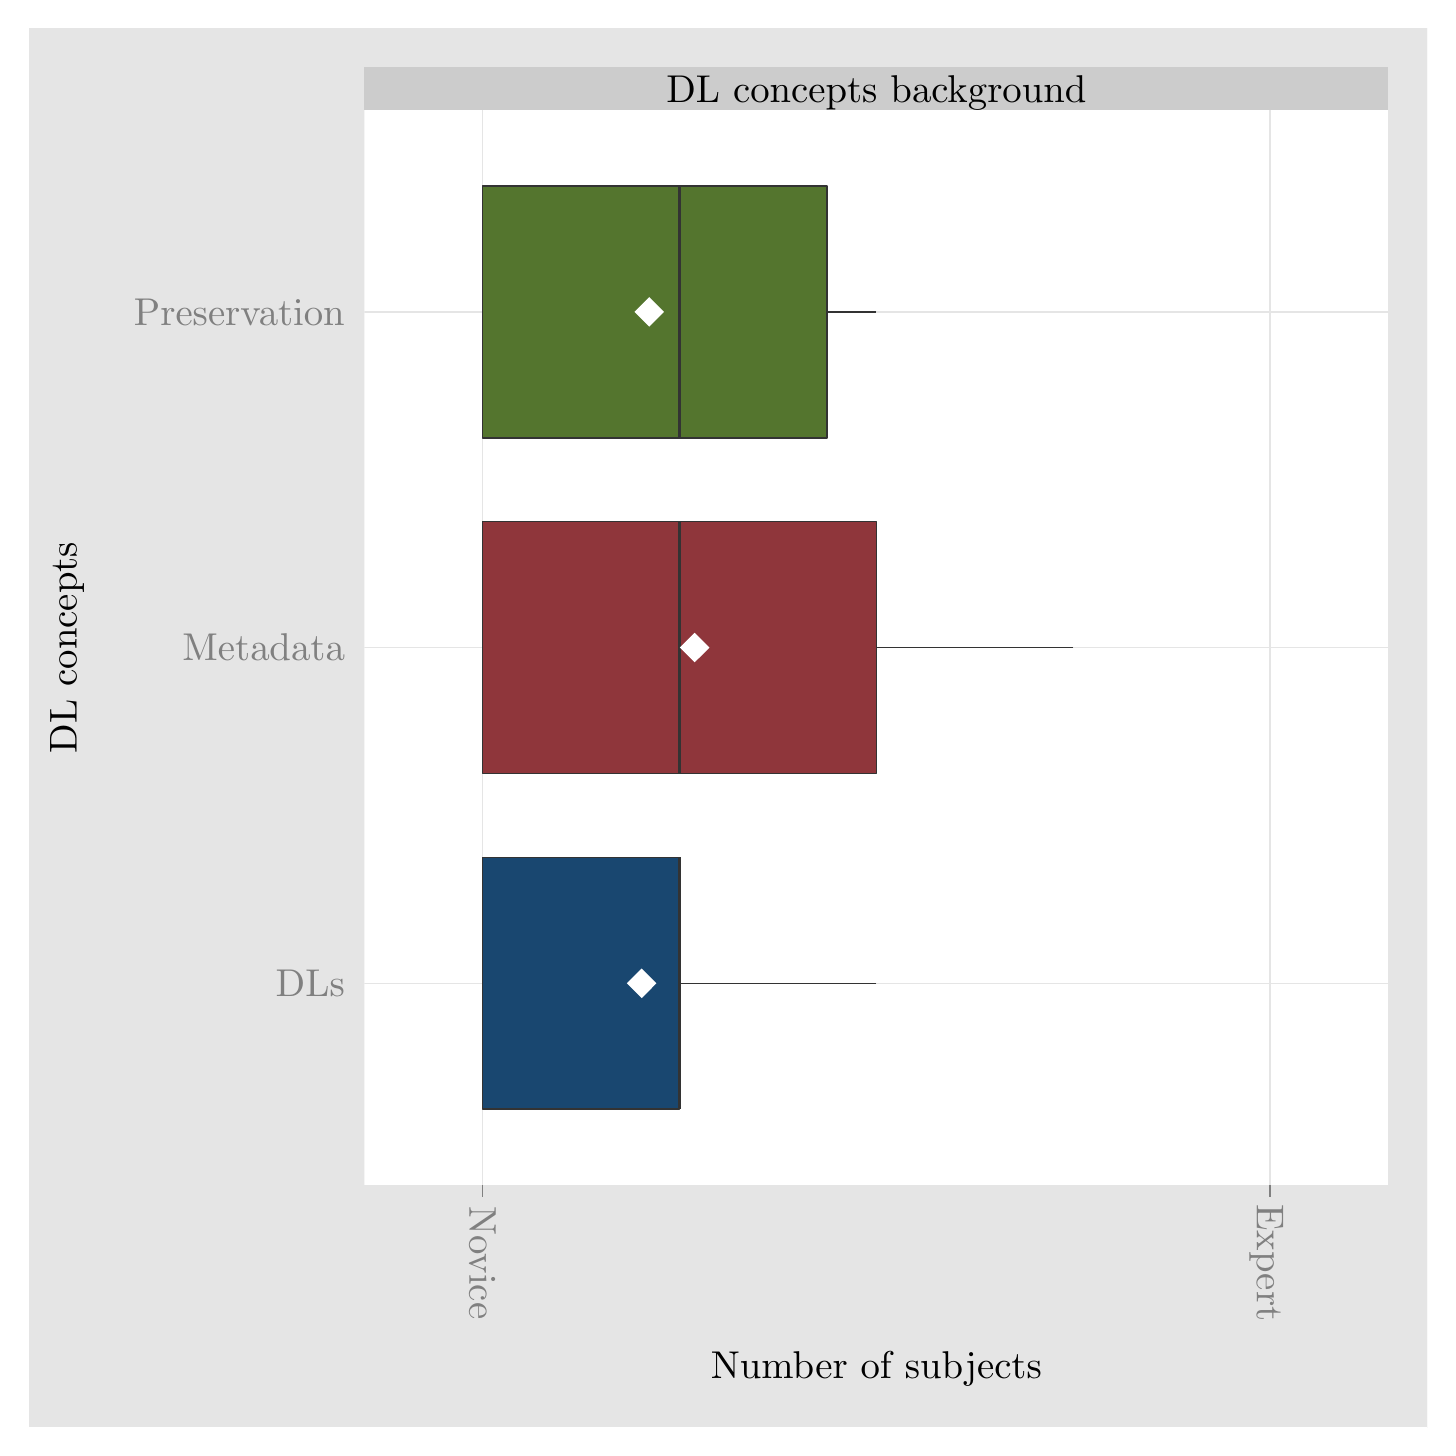
\begin{tikzpicture}[x=1pt,y=1pt]
\definecolor[named]{fillColor}{rgb}{1.00,1.00,1.00}
\path[use as bounding box,fill=fillColor,fill opacity=0.00] (0,0) rectangle (505.89,505.89);
\begin{scope}
\path[clip] (  0.00,  0.00) rectangle (505.89,505.89);
\definecolor[named]{drawColor}{rgb}{1.00,1.00,1.00}
\definecolor[named]{fillColor}{rgb}{0.90,0.90,0.90}

\path[draw=drawColor,line width= 0.6pt,line join=round,line cap=round,fill=fillColor] (  0.00, -0.00) rectangle (505.89,505.89);
\end{scope}
\begin{scope}
\path[clip] (121.70, 87.76) rectangle (491.66,476.00);
\definecolor[named]{fillColor}{rgb}{1.00,1.00,1.00}

\path[fill=fillColor] (121.70, 87.76) rectangle (491.66,476.00);
\definecolor[named]{drawColor}{rgb}{0.90,0.90,0.90}

\path[draw=drawColor,line width= 0.6pt,line join=round] (121.70,160.56) --
	(491.66,160.56);

\path[draw=drawColor,line width= 0.6pt,line join=round] (121.70,281.88) --
	(491.66,281.88);

\path[draw=drawColor,line width= 0.6pt,line join=round] (121.70,403.20) --
	(491.66,403.20);

\path[draw=drawColor,line width= 0.6pt,line join=round] (164.39, 87.76) --
	(164.39,476.00);

\path[draw=drawColor,line width= 0.6pt,line join=round] (448.98, 87.76) --
	(448.98,476.00);
\definecolor[named]{drawColor}{rgb}{0.20,0.20,0.20}
\definecolor[named]{fillColor}{rgb}{0.20,0.20,0.20}

\path[draw=drawColor,line width= 0.6pt,line join=round,fill=fillColor] (235.54,160.56) -- (306.68,160.56);

\path[draw=drawColor,line width= 0.6pt,line join=round,fill=fillColor] (164.39,160.56) -- (164.39,160.56);
\definecolor[named]{fillColor}{rgb}{0.10,0.28,0.44}

\path[draw=drawColor,line width= 0.6pt,line join=round,line cap=round,fill=fillColor] (235.54,115.06) --
	(164.39,115.06) --
	(164.39,206.05) --
	(235.54,206.05) --
	(235.54,115.06) --
	cycle;
\definecolor[named]{fillColor}{rgb}{0.20,0.20,0.20}

\path[draw=drawColor,line width= 1.1pt,line join=round,fill=fillColor] (235.54,115.06) -- (235.54,206.05);

\path[draw=drawColor,line width= 0.6pt,line join=round,fill=fillColor] (306.68,281.88) -- (377.83,281.88);

\path[draw=drawColor,line width= 0.6pt,line join=round,fill=fillColor] (164.39,281.88) -- (164.39,281.88);
\definecolor[named]{fillColor}{rgb}{0.56,0.21,0.23}

\path[draw=drawColor,line width= 0.6pt,line join=round,line cap=round,fill=fillColor] (306.68,236.38) --
	(164.39,236.38) --
	(164.39,327.38) --
	(306.68,327.38) --
	(306.68,236.38) --
	cycle;
\definecolor[named]{fillColor}{rgb}{0.20,0.20,0.20}

\path[draw=drawColor,line width= 1.1pt,line join=round,fill=fillColor] (235.54,236.38) -- (235.54,327.38);

\path[draw=drawColor,line width= 0.6pt,line join=round,fill=fillColor] (288.90,403.20) -- (306.68,403.20);

\path[draw=drawColor,line width= 0.6pt,line join=round,fill=fillColor] (164.39,403.20) -- (164.39,403.20);
\definecolor[named]{fillColor}{rgb}{0.33,0.46,0.18}

\path[draw=drawColor,line width= 0.6pt,line join=round,line cap=round,fill=fillColor] (288.90,357.71) --
	(164.39,357.71) --
	(164.39,448.70) --
	(288.90,448.70) --
	(288.90,357.71) --
	cycle;
\definecolor[named]{fillColor}{rgb}{0.20,0.20,0.20}

\path[draw=drawColor,line width= 1.1pt,line join=round,fill=fillColor] (235.54,357.71) -- (235.54,448.70);
\definecolor[named]{fillColor}{rgb}{1.00,1.00,1.00}

\path[fill=fillColor] (216.52,160.56) --
	(221.86,165.89) --
	(227.19,160.56) --
	(221.86,155.22) --
	cycle;

\path[fill=fillColor] (235.68,281.88) --
	(241.01,287.22) --
	(246.35,281.88) --
	(241.01,276.55) --
	cycle;

\path[fill=fillColor] (219.26,403.20) --
	(224.59,408.54) --
	(229.93,403.20) --
	(224.59,397.87) --
	cycle;
\end{scope}
\begin{scope}
\path[clip] (  0.00,  0.00) rectangle (505.89,505.89);
\definecolor[named]{fillColor}{rgb}{0.80,0.80,0.80}

\path[fill=fillColor] (121.70,476.00) rectangle (491.66,491.66);
\definecolor[named]{drawColor}{rgb}{0.00,0.00,0.00}

\node[text=drawColor,anchor=base,inner sep=0pt, outer sep=0pt, scale=  1.40] at (306.68,479.01) {DL concepts background};
\end{scope}
\begin{scope}
\path[clip] (  0.00,  0.00) rectangle (505.89,505.89);
\definecolor[named]{drawColor}{rgb}{0.50,0.50,0.50}

\node[text=drawColor,anchor=base east,inner sep=0pt, outer sep=0pt, scale=  1.40] at (114.59,155.74) {DLs};

\node[text=drawColor,anchor=base east,inner sep=0pt, outer sep=0pt, scale=  1.40] at (114.59,277.06) {Metadata};

\node[text=drawColor,anchor=base east,inner sep=0pt, outer sep=0pt, scale=  1.40] at (114.59,398.38) {Preservation};
\end{scope}
\begin{scope}
\path[clip] (  0.00,  0.00) rectangle (505.89,505.89);
\definecolor[named]{drawColor}{rgb}{0.50,0.50,0.50}

\path[draw=drawColor,line width= 0.6pt,line join=round] (164.39, 83.49) --
	(164.39, 87.76);

\path[draw=drawColor,line width= 0.6pt,line join=round] (448.98, 83.49) --
	(448.98, 87.76);
\end{scope}
\begin{scope}
\path[clip] (  0.00,  0.00) rectangle (505.89,505.89);
\definecolor[named]{drawColor}{rgb}{0.50,0.50,0.50}

\node[text=drawColor,rotate=270.00,anchor=base,inner sep=0pt, outer sep=0pt, scale=  1.40] at (159.57, 59.54) {Novice};

\node[text=drawColor,rotate=270.00,anchor=base,inner sep=0pt, outer sep=0pt, scale=  1.40] at (444.15, 59.54) {Expert};
\end{scope}
\begin{scope}
\path[clip] (  0.00,  0.00) rectangle (505.89,505.89);
\definecolor[named]{drawColor}{rgb}{0.00,0.00,0.00}

\node[text=drawColor,anchor=base,inner sep=0pt, outer sep=0pt, scale=  1.40] at (306.68, 17.94) {Number of subjects};
\end{scope}
\begin{scope}
\path[clip] (  0.00,  0.00) rectangle (505.89,505.89);
\definecolor[named]{drawColor}{rgb}{0.00,0.00,0.00}

\node[text=drawColor,rotate= 90.00,anchor=base,inner sep=0pt, outer sep=0pt, scale=  1.40] at ( 17.70,281.88) {DL concepts};
\end{scope}
\end{tikzpicture}
